\chapter{Detecția și izolarea defectelor}
\label{chap:detectie}
\section{Definirea defectelor}
Defectele sunt simulate modificând parametrul $C$ din ecuația emitter-ului \eqref{eq:emitter}. Modalitatea prin care se execută în cod simularea unui defect este prin apelarea metodei:

\lstinputlisting[language=Python, caption={Funcție pentru simularea defectelor},label={lst:set_emitter}, firstline=23,lastline=26]{\code/ENWrapper.py}

parametrii funcției $set_emitter$ sunt:
\begin{itemize}
\item node\_inde - indexul nodului în care se simulează defectul
\item emitter\_val - magnitudinea defectului
\end{itemize}

Metoda mai întâi vefică dacă nodul cu indexul $node_index$ reprezintă doar o jonncțiune apoi setează magnitudinea defectului în nodul primit cu ajutorul funcției de bibliotecă $\mathbf{ENsetnodevalue}$ 

\section{Simulare dinamică pentru defecte în diferite noduri}

În continuare vom considera un scenariu de defect pentru rețea care constă în modificarea succesivă a parametrului de proporționalitate din relația de calcul a debitului de emitter \eqref{eq:emitter}. În imaginile următoare voi considera mai multe magnitudini de defect într-un anumit nod și voi reprezenta grafic răspunsul în timp al rețelei în același nod.

\begin{figure}[H]

\subfloat[Profile cu defect în nodul 14]{%
  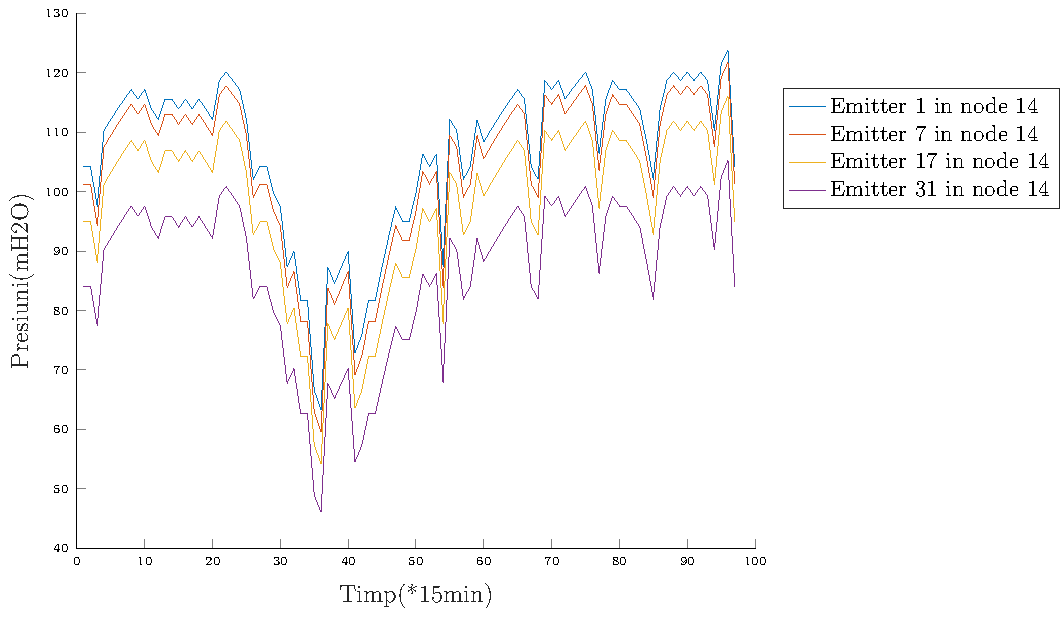
\includegraphics[width=0.5\textwidth]{\pics/c2_pics/emitter_node_same/emitter_node14}%
  \label{fig:emitter_node_same14}%
}\qquad
\subfloat[Profil cu defect în nodul 25]{%
  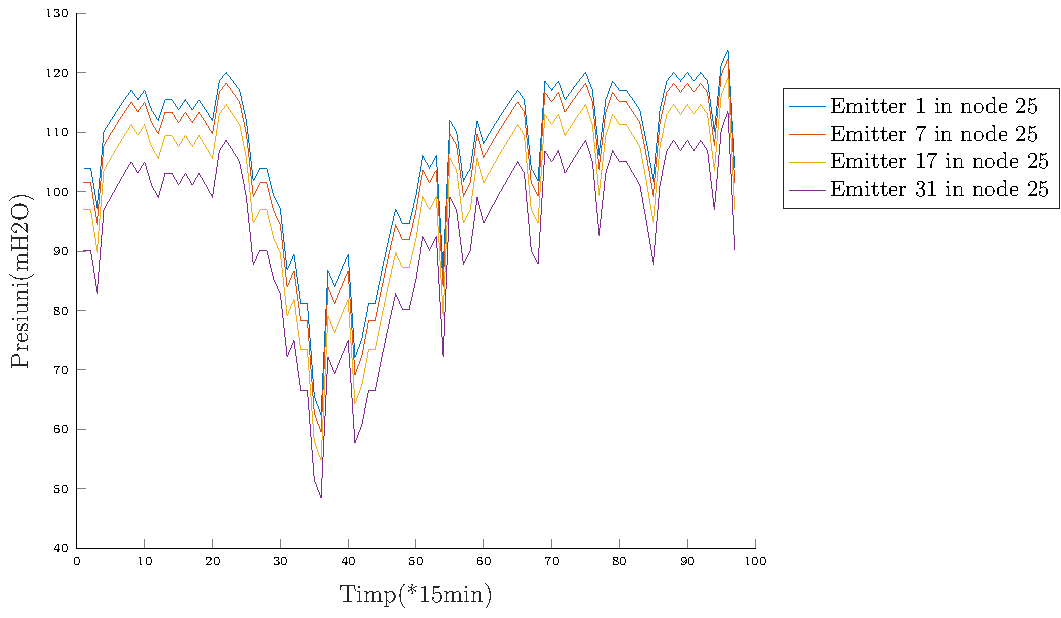
\includegraphics[width=0.5\textwidth]{\pics/c2_pics/emitter_node_same/emitter_node25}%
  \label{fig:emitter_node_same25}\qquad
}

\caption{Rezultate simulări defecte ușoare}
\label{fig:ref_emitter_soft}
\end{figure}

După cum se poate observa în imaginile \ref{fig:ref_emitter_soft} variația emitter-ului într-un nod produce în mod evident o modificarea a modului comun al caracteristicii $timp-presiune$. Din punctul de vedere al magnitudinolor de simulare pentru defecte, am considerat 2 clase de defecte, anume:
\begin{itemize}
\item defecte ușoare (soft faults) - cu valorile coeficientului de emitter mai mici de 35
\item defecte puternice (hard faults) - cu valorile emitter mai mari de 35 
\end{itemize}

Cele din urmă produc și modificări ale caracteristicii dinamice, introducând distorsiuni sau aplatizări ale mărimilor măsurate. Reprezentarea defectelor hard este reprezentată în figurile de mai jos:

\begin{figure}[H]

\subfloat[Profile cu defect puternic în nodul 14]{%
  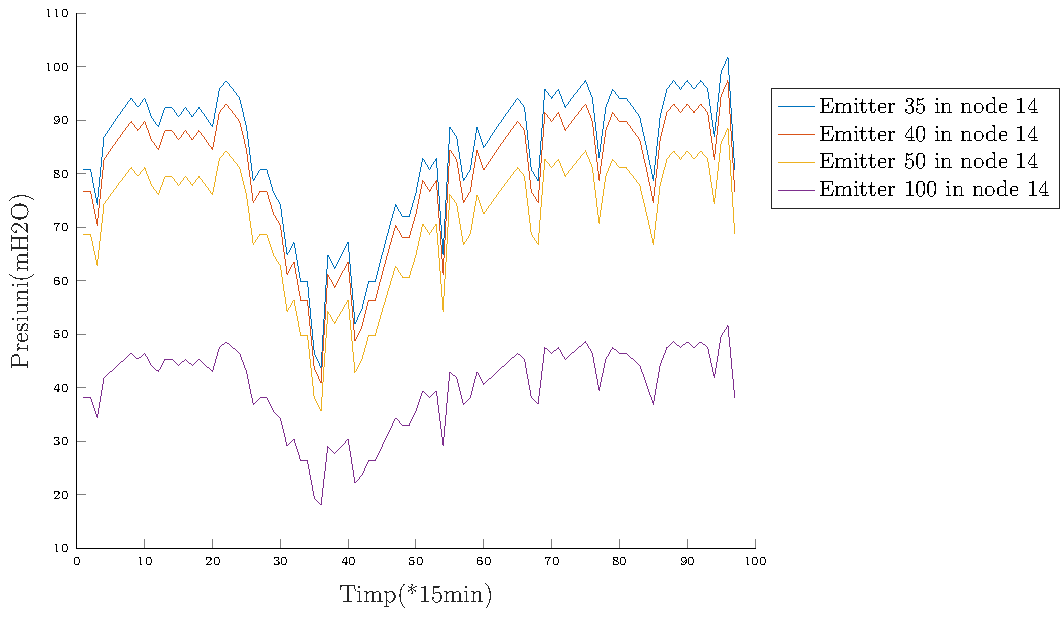
\includegraphics[width=0.5\textwidth]{\pics/c2_pics/emitter_node_same/emitter_hard_node14}%
  \label{fig:emitter_hard_node_same14}%
}\qquad
\subfloat[Profil cu defect puternic în nodul 25]{%
  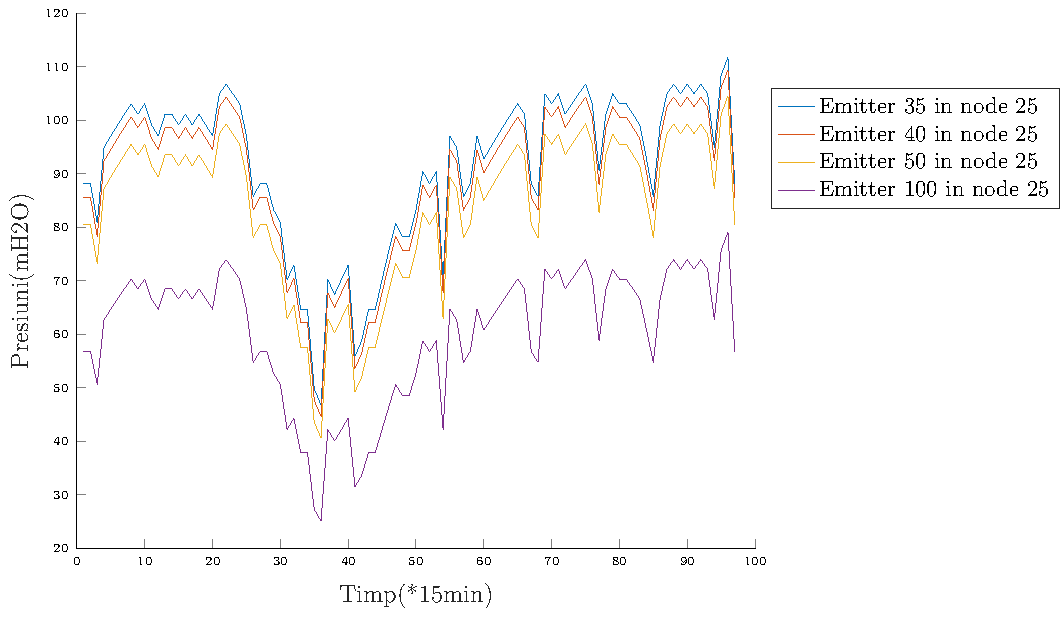
\includegraphics[width=0.5\textwidth]{\pics/c2_pics/emitter_node_same/emitter_hard_node25}%
  \label{fig:emitter_hard_node_same25}\qquad
}

\caption{Rezultate simulări defecte puternice}
\label{fig:ref_emitter_hard}
\end{figure}

Se observă de exemplu că pentru o valoare a emitter-ului de 100 caracteristica dinamică este deja modificată din cauza scurgerilor puternice din nod. 

Este relevantă împărțirea defectelor în mai multe clase de magnitudini pentru a putea valida un model de clasificare. Spre exemplu este normal să se întrebe dacă un model antrenat pe baza unui set date corespunzător unor magnitudini normale $C \in (0, 35)$ poate da rezultate semnificative pentru un set de date cu magnitudini ale emitter-ului puternice $C \geqslant 35$. 

\section{Preprocesare datelor}
În urma extragerii datelor din rețea este extrem de importantă etapa de prelucrare și preprocesare a datelor. Domeniul de preprocesare a datelor este unul extrem de vast 

